% Template:     Auxiliar LaTeX
% Documento:    Archivo principal
% Versión:      8.3.3 (20/01/2025)
% Codificación: UTF-8
%
% Autor: Pablo Pizarro R.
%        pablo@ppizarror.com
%
% Manual template: [https://latex.ppizarror.com/auxiliares]
% Licencia MIT:    [https://opensource.org/licenses/MIT]

% CREACIÓN DEL DOCUMENTO
\documentclass[
	spanish, % Idioma: spanish, english, etc.
	letterpaper, oneside
]{article}

% INFORMACIÓN DEL DOCUMENTO
\def\documenttitle {Auxiliar 5}
\def\documentsubject {Dinámica}

\def\documentauthor {Nombre del autor}
\def\coursename {Mecánica}
\def\coursecode {FI-2001}

\def\universityname {Universidad de Chile}
\def\universityfaculty {Facultad de Ciencias Físicas y Matemáticas}
\def\universitydepartment {Departamento de la Física}
\def\universitydepartmentimage {departamentos/fcfm}
\def\universitydepartmentimagecfg {height=1.75cm}
\def\universitylocation {Santiago de Chile}

% EQUIPO DOCENTE
\def\teachingstaff {
	\textbf{Profesor: Simón Riquelme} \\
	Auxiliares: Jorge Barja, Ian Tobar \\
	Ayudante: Matías Abrigo  \\
}

% IMPORTACIÓN DEL TEMPLATE
\input{template}

% INICIO DE PÁGINAS
\begin{document}

% CONFIGURACIÓN DE PÁGINA Y ENCABEZADOS
\templatePagecfg

% ======================= INICIO DEL DOCUMENTO =======================

% \newboxquestion{P1}\\

% Considere una bolita de masa $m$ ensartada en una barra de manera que puede deslizar sin roce por ella. La masa está atada mediante un resorte, de constante elástica $k$ y largo natural $l_0$, a un extremo de la barra, y esta última, a su vez, gira c/r al mismo extremo en un plano horizontal con velocidad angular $w$ constante. En $t=0$ la bolita se suelta con resorte comprimido en $l_0/2$ y $\dot{\rho}(0) = 0$:

% \begin{enumerate}[label=\alph*)]
%     \item ¿Qué relación deben cumplir $m,k$ y $w$ para que la bolita realice un movimiento armónico simple a lo largo de la barra?.
%     \item Determine la compresión del resorte como función del tiempo..

% \end{enumerate}


% \begin{figure}[ht] % [h] indica que se coloca la imagen aquí (here)
%     \centering % Centra la imagen
%     
\includegraphics[width=0.4\textwidth]{p1.png} % Ajusta el tamaño de la imagen
%     \caption{Pregunta 1.} % Subtítulo de la imagen
%     \label{fig:p1} % Etiqueta opcional para referencias
% \end{figure}

\newboxquestion{P1}\\

Una barra gira con velocidad angular constante $w_0$ respecto de un punto $O$ bajo la influencia del campo gravitacional, manteniéndose siempre en un mismo plano vertical. Encima de la barra desliza una partícula de masa $m$ sobre la cual actúa una fuerza motriz radial $F = F(t)\hat r$. En el movimiento resultante de la partícula, esta se desplaza con rapidez constante $v_0$ respecto de la barra, como muestra la figura. Considere que la barra es infinitamente larga y desprecie todo roce.

\begin{enumerate}[label=\alph*)]
    \item Determine el valor mínimo de $v_0$ tal que la partícula nunca se despegue de la barra.
    
    \item Si $v_0$ tiene el valor obtenido en $(a)$, determine la fuerza $F$ en función del tiempo: $F(t)$. Considere que en $t=0$ la barra pasa por la horizontal y la partícula pasa por el punto $O$.
    
    \item Determine el ángulo $\theta$ que forma la barra con la horizontal cuando $F$ alcanza su mayor valor positivo. (propuesto)
    Sol: $\theta = \pi/3$

\end{enumerate}
\textbf{Hint:} Puede ser útil recordar que $sen(arc \space cos(x)) = \sqrt{1 - x^2}$

\begin{figure}[ht] % [h] indica que se coloca la imagen aquí (here)
    \centering % Centra la imagen
    \hspace{-1.5cm} % Desplaza la imagen 2 cm a la izquierda
    
\includegraphics[width=0.5\textwidth]{p2.png} % Ajusta el tamaño de la imagen
    \caption{Pregunta 1.} % Subtítulo de la imagen
    \label{fig:p2} % Etiqueta opcional para referencias
\end{figure}

\newboxquestion{P2} ($\star$) \\

Un Casquete semi-esferico de radio $R$ tiene un orificio pequeño en su parte superior. Por él, pasa una cuerda ideal inextendible de largo $\pi R/2$ con dos masas identicas $m$ en sus extremos. Una de las masas cuelga verticalmente desde el orificio, mientras que la otra siempre pertenece en contacto con la superficie del casquete. Inicialmente, la masa sobre el casquete es tal que $\theta_0=\pi /4$, $\dot{\theta} = 0$, $\phi_0 = 0$ y $\dot{\phi} = w_0$.

\begin{enumerate}[label=\alph*)]
    \item Encuentre las ecuaciones de movimiento.
    %Sol: $ v(\theta) = \frac{\sin\theta}{\sqrt{5 + 4\cos \theta}}v_0 $
    \item Encuentre dependencia de $ \dot\phi$ con respecto a $\theta$.
    %Sol: $ \vec{v}_{max} = \pm \frac{v_0}{2} \hat{k}$
    \item Encontrar ecuación del estilo $f(\theta, \dot\theta,\ddot \theta) = 0$ (propuesto).
    %Sol: $ \vec{a}(\theta = 0) = - \frac{v^2_0}{3R} \hat{k}$
\end{enumerate}

\begin{figure}[ht] % [h] indica que se coloca la imagen aquí (here)
    \centering % Centra la imagen
    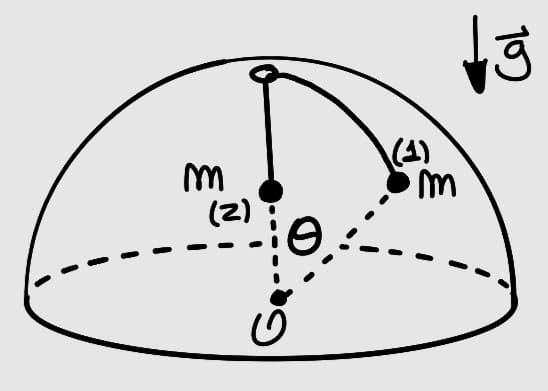
\includegraphics[width=0.4\textwidth]{p3.jpeg} % Ajusta el tamaño de la imagen
    \caption{Pregunta 2.} % Subtítulo de la imagen
    \label{fig:p3} % Etiqueta opcional para referencias
\end{figure}



\newboxquestion{P3}\\


Hay un hilo enrollado alrededor de un cilindro de radio R. En la punta del hilo hay un cuerpo de masa $m$ que se suelta,cuando $\phi =0$, con velocidad inicial $\vec{v}(t=0)=-v_0\hat{\rho}$, perpendicular al hilo, lo que determina que el hilo se comienza a enrollar. La distancia inicial entre el cuerpo y el punto B de tangencia del hilo con el cilindro es $L_0$. \textbf{No hay gravedad.}

\noindent \textbf{Nota:} Las coordenadas cilíndricas en este problema persiguen al punto de tangencia B, y es conveniente escribir el vector posición como: $\vec{r} = R\hat{\rho} + L(t)\hat{\phi}$.

\begin{enumerate}[label=\alph*)]
    \item Determine la ecuación de movimiento para la distancia $L(t)$ correspondiente a la longitud de hilo que queda por enrollar en el tiempo t (distancia entre los puntos B y la posición de la masa).
    \item Obtenga la velocidad angular $\dot{\phi}$ en función de $\phi$.
    \item Suponiendo que el hilo se corta si la tensión sobrepasa el valor $T_{max}$, obtenga el valor de $\phi$ en el momento del corte (propuesto).
\end{enumerate}

\begin{figure}[ht]
    \centering
    % Primera imagen
    \begin{subfigure}[b]{0.24\textwidth}
        \centering
        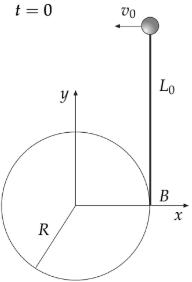
\includegraphics[width=\textwidth]{p4a.png}
        %\caption{Subtítulo de la segunda imagen}
        \label{fig:imagen1}
    \end{subfigure}
    \hspace{1.0 cm} % Espacio entre las imágenes
    % Segunda imagen
    \begin{subfigure}[b]{0.24\textwidth}
        \centering
        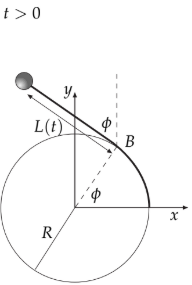
\includegraphics[width=\textwidth]{p4b.png}
        %\caption{Subtítulo de la segunda imagen}
        \label{fig:imagen2}
    \end{subfigure}
    \caption{Pregunta 3.}
    \label{fig:imagenes}
\end{figure}

\newboxquestion{P4} \textbf{(Propuesto)}\\

Un anillo de radio $R$ gira con velocidad angular 
$\vec{\omega}_\phi = \omega_\phi \hat{k}$ en torno al eje vertical $z$ de la figura, 
el cual pasa por su centro en el punto $O$ y se intersecta con el anillo en los puntos 
$A$ y $B$. La velocidad angular $\omega_\phi$ \textbf{no} es necesariamente constante. 
Otro anillo mucho más pequeño, de masa $m$, desliza sin roce y en presencia de 
aceleración de gravedad $\vec{g} = - g \hat{k}$ a lo largo del anillo de radio $R$. 
La posición del anillo pequeño está determinada por el ángulo $\theta$ que se muestra 
en la figura. \\

\begin{minipage}{0.65\textwidth}

\begin{enumerate}[label=\alph*)]
    \item Encuentre el valor de $\omega_\phi$ en función de $\theta$ 
    (es decir, $\omega_\phi(\theta)$) de modo que $\dot{\theta}$ sea constante en todo 
    instante. Determine el rango para $\theta$ en el cual esto es posible.\\
    Sol: $w_\phi^2 = -\frac{g}{Rcos(\theta)}$

    \item Si se sabe que en todo instante 
    $\dot{\theta} = \sqrt{g/R}$, y considerando la fuerza normal $\vec{N}$ que ejerce 
    el anillo de radio $R$ sobre el anillo pequeño, encuentre su componente radial 
    $N_r = \hat{r} \cdot \vec{N}$ en términos de $m$, $g$ y $\theta$.\\
    Sol: $N_r = mg(1 - \frac{1}{cos(\theta)})$
\end{enumerate}
\end{minipage}
\hfill
\begin{minipage}{0.3\textwidth}
\centering

\includegraphics[width=\linewidth]{p5.png}
\end{minipage}

% FIN DEL DOCUMENTO
\end{document}